\documentclass{article}
\usepackage[utf8]{inputenc}

\title{Efficient Estimation of Word Representations in Vector Space}
\author{}
\date{}

\usepackage{natbib}
\usepackage{graphicx}
\usepackage{amsmath}
\usepackage[left=2.5cm,right=2.5cm,top=1cm,bottom=1.25cm]{geometry}
\usepackage{hyperref}
\usepackage{float}
\usepackage[export]{adjustbox}



\hypersetup{colorlinks=true,urlcolor=blue}
\pagenumbering{gobble}

\begin{document}

\maketitle

\section*{Link}
\href{https://arxiv.org/abs/1301.3781}{arXiv} 

\section*{Summary}
\begin{itemize}
    \item Distributed representations of words learned by neural networks usually perform better than other approaches. Traditional approach to this used feedforward neural network language model (NNLM) or recurrent neural net language model (RNNLM). NNLM has computation complexity of $N\times D \times + N \times D \times H + H \times V$ and RNNLM has computation complexity of $H \times H + H \times V$ where $H$ is hidden layer dimension, $V$ is vocabulary size. When we use hierarchical softmax the number of outputs we need to evaluate can go down to $log_2(V)$. So most of the complexity is caused by non-linear hidden layer. 
    \item This paper uses couple of simple architectures to learn word embedding that don't use hidden layer. This enables them to use higher dimensional embedding and train on larger dataset.
    \begin{enumerate}
        \item First approach is continuous bag-of-words(CBOW) model. In this approach $N$ surrounding words is used to predict the center word. They obtained best result by using four past and four future words. Computation complexity is $N \times D + D \times log_2(V)$.
        \item In continuous skip=gram model, the center word is used to predict the surrounding words. Since more distant words are usually less similar to current word, less weight is given to the distant words by sampling less from those. The computation complexity is $C\times D + C \times D \times log_2(V)$.
    \end{enumerate}
    \begin{figure}[H]
        \centering
        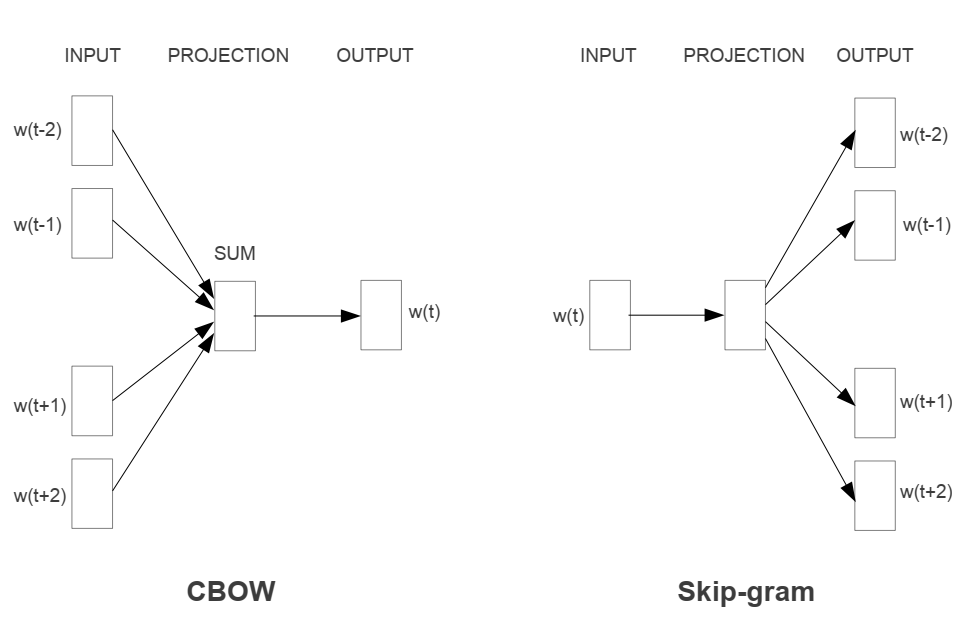
\includegraphics[scale=0.5]{architectures.png}
        \caption{CBOW and skip-gram architectures}
        \label{fig:Figure 1}
    \end{figure}
    \item To evaluate performance, they denote two pairs of words with the same relationship as a question, asking "What is the word that is similar to \textit{small} in the same sense as \textit{biggest} is similar to \textit{big}?" This can be answered by simple algebraic operations on vector representation of words. To answer the above question we can simply calculate the vector $X=vector("biggest")-vector("big")+vector("small")$. We can then search in the vector space for the word closest to $X$ measured by cosine distance and use it as the answer to the question. 
    \item When we train on larger dataset, we should use higher dimensional vector otherwise the gain in performance won't be significant.
    \item Skip-gram model was able to capture better semantic relationship between words than other approaches. Both CBOW and Skip-gram perform comparatively to NNLM model on syntactic similarity task but require much less time to train.
    \item To improve accuracy on the word similarity task, we can provide more than one example of the relationship. By using ten examples instead of one to form the relationship vector (averaging the individual vectors together) they were able to improve accuracy by 10\%.
    \item We can also find out out-of-the-list words by computing average vector for a list of words and finding the most distant word vector.

\end{itemize}

\end{document}
